\documentclass[a4paper, 10pt]{IEEEtran}
\usepackage[utf8]{inputenc}

\title{\LARGE Program Comprehension, Obfuscation, and Style Guides: A Survey of Code Confusion}
\author{David Stout}
\date{September 2018}

%\usepackage{natbib}
\usepackage{graphicx}

\begin{document}

\maketitle
\begin{abstract}
Rough Draft, and will continue to flesh out the key areas in the upcoming weeks.
\end{abstract}
\section{Introduction}
\begin{quote}
    "We often confuse what we wish for with what is." - Neil Gaiman
\end{quote}


Confusion is something that everyone faces in life at some point, whether it is rooted in unclear instructions, convoluted rules, or the actions of others, confusion is an obstacle that must be overcome to achieve the goals we want. Zokaites \cite{zokaites_writing_2002} describes software as a natural language that must be understood by two separate entities for two different purposes. One being the compiler/interpreter that transfers source code into machine language, and the other being people that need to maintain, utilize and develop the application. Code confusion is when people, whether by design or by happenstance, misunderstand the functionality or intent of source code sections. 

Computer science is no stranger to confusing code, and sometimes the intent is to make code inherently confusing by obfuscating it for security and privacy. While we will have no issues with compilers and interpreters handling confusing code, we run into issues when developers are attempting to debug, re-factor, and maintain source code. Code confusion creates an expensive overhead cost to developers and is an acknowledged problem in the community that has had a number of suggested solutions proposed, but has never had a panacea solution.

This survey will explore the effectiveness of the methods suggested by the analysis of program comprehension, obfuscation (and concurrently de-obfuscation), and style guides. Analysis of the methods that are currently available will show that there is still room for newer methods of identification and solutions to make source code much less confusing.

\begin{figure}[ht!]
\centering
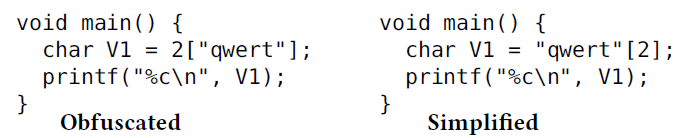
\includegraphics[scale=0.45]{Confusing_Code.PNG}
\caption{Atom of Confusion example from Gopstein et al.}
\label{fig:Atom}
\end{figure}

\newpage
\section{Classification Model}
\begin{figure}[ht!]
\centering
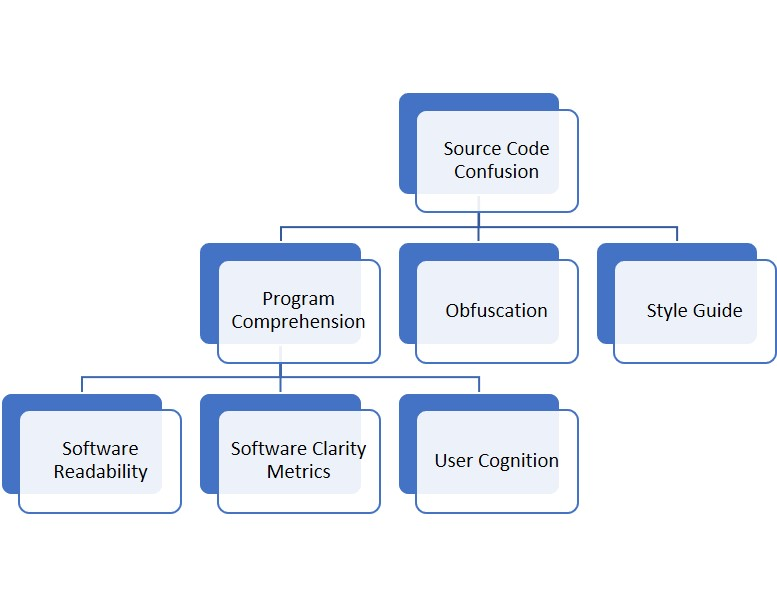
\includegraphics[scale=0.45]{Classification_Model}
\caption{Classification Model of Paper Hierarchy}
\label{fig:Classification}
\end{figure}

\section{Papers list}

\subsection{Program Comprehension}

\begin{itemize}
    \item \textbf{\textit{“Towards a theory of the comprehension of computer programs"}}
    This older theory paper explains the process that a developer goes through to comprehend source code, starting to define program comprehension. It is an older paper, so the issue of program comprehension has been around for decades. Field has moved beyond it, but the paper gives a good starting point for the issue at hand being one that is still relevant.
    \item \textbf{\textit{“On the Comprehension of Program Comprehension"}}
    Paper finds that programmers tend to shy away from comprehension methods unless pressed, often choosing to put themselves in the role of the user instead. Comprehension tools while being available seem to not be used as much in practice, begging the question are the tools doing what we need them to be or do they simply not have enough widespread exposure for acceptance.
    \item \textbf{\textit{“How do professional developers comprehend software?"}}
    Paper seeks to identify what methods, strategies and tools are used by professional developers when in industry. By identifying the methods that pros are actually using, refinement of research and tools can be made. I think it is always best to get info from working professionals to determine usefulness of research, who cares if you have the most efficient tool for the job if no one wants to use it.
\end{itemize}
\subsubsection{Software Readability}
\begin{itemize}
    \item \textbf{\textit{“Writing Understandable Code"}}
    This article talks about the benefits of commenting for for future readability. While in some situations comments are a welcome addition to readability of complex functions and algorithms, too many comments can adversely affect readability. I believe that this paper's recommendations should be taken lightly, and used sparingly.
    \item \textbf{\textit{“Understanding  misunderstandings  in  source  code"}}
This theoretical paper addresses the problem of developer misunderstandings in source code that affect software readability. The solution that is presented is that the confusing code can be identified and future style guides/standards may be written with non-confusing patterns instead to increase software readability. The paper    creates a new taxonomy for confusing code called "atoms of confusion", new classification creates a lot of room for future research.
    \item \textbf{\textit{“Tool assisted identifier naming for improved software readability"}}
    This paper presents a code editor that offers dynamic feedback to the developer on identifier naming practices to improve code readability during development process. Presents an approach that was shown to benefit both novices and skilled programmers. Possible that proper identifier naming can be combined with other methods to increase readability.
    \item \textbf{\textit{“Supporting program comprehension with source code summarization"}}
    Use of summarization to increase the readability and comprehension of larger scale projects. Proposes an automated text summarization technology to reduce source code entities to simple code semantics. Concept maybe useful on larger scale project to perform follow up experimentation, without users easily experiencing fatigue.
    \item \textbf{\textit{“Relating identifier naming flaws and code quality"}}
    Workshop that explores if bad identifier names effect code readability, thus impacting maintenance. Improper identifier names were found to significantly impact code quality using static analysis tools. Findings enhance previous experimentation in identifier naming. 
    \item \textbf{\textit{“Prevalence of confusing code in software projects: atoms of confusion in the wild"}}
    Follow up paper to previous work in Atoms of confusion. Paper identifies 15 determined confusing micropatterns of confusing code that occur numerous times in large scale open-source production code. Only 15 identified in this paper, but the potential for many more confusing micropatterns being in use is high. 
    \item \textbf{\textit{“Exploring the influence of identifier names on code quality: An empirical study"}}
    Paper builds on previous work that found a connection between identifier name quality and overall software quality when using static analysis. Paper shows that bad identifier names impact the quality of Java methods and impact readability metrics. Refining the particular identifier naming flaws will help to identify problems in program comprehension for maintenance.

\item \textbf{\textit{“Evaluating the Quality of Open Source Software"}}
    As the landscape of programming has changed with the emergence of more open-source projects, it has opened the opportunity to examine these projects for software quality. This in turn is indicative of the software readability of programmers in projects outside of the traditional industry settings. When rules may be lax, do the developers still attempt to integrate software readability practices to ensure program comprehension for potentially new developers. 

\end{itemize}
\subsubsection{User Cognition}
\begin{itemize}
    \item \textbf{\textit{“Understanding Understanding source code with functional MRI"}}
    Paper maps the areas of the brain that fire when looking at source code to map cognitive processes during program comprehension. The experiment shows that 5 areas of the brain fire during code comprehension exercises. The measurement technique could be useful to examine what coding methods will yield the best results for software readability.
    \item \textbf{\textit{“Quantifying programmers' mental workload during program comprehension based on cerebral blood flow measurement"}}
    Paper uses measured cerebral blood flow during program comprehension exercises to determine programmers' mental workload. Measurement of workload during program comprehension could lead to identifying methodologies that are better suited for developers based on cognition. 
    \item \textbf{\textit{“Measuring neural efficiency of  program  comprehension"}}
    Paper builds on author's earlier work in measuring cognitive effectiveness during program comprehension. Experiment uses bottom-up chunking and semantic cues, in beacons, to determine a more efficient method for software readability. Limited scope of experiment leaves room for other methods to be applied in future research.
    \item \textbf{\textit{“Detecting and comparing brain activity in short program comprehension using EEG"}}
    Paper seeks to provide a method for measuring cognition during program comprehension of predetermined confusing and non-confusing code snippets by measuring brain wave patterns. Accurately measuring user cognition in program comprehension can help to identify which methods of supporting software readability are most worthwhile. Results are promising and merit further research

\end{itemize}
\subsubsection{Software Clarity Metrics}
\begin{itemize}
    \item \textbf{\textit{“Learning a Metric for Code Readability"}}
    The approach of this paper is to identify a method of automating code analysis for measuring software readability to give an indication of software quality and maintainability. The solution presented is not something that is intended as the final measure of readability.
    \item \textbf{\textit{“A Simpler Model of Software Readability"}}
    Paper model uses well-known size metrics and Halstead metrics, which are easily extracted using
    a variety of tools, to build on the method of automating code analysis to measure software readability. While readability may be somewhat subjective, the paper offers a set of metrics that are useful for automating the analysis of code to return some credible results. If developers want to reduce costs in both initial development and maintenance, then automated testing suites will be necessary. 
\end{itemize}

\subsection{Obfuscation}
\begin{itemize}
    \item \textbf{\textit{“The effectiveness of source code obfuscation"}}
    Explores source code intentional obfuscation to limit the likelihood of reverse engineering. Process is the reverse of readability, which could provide further insight into comprehension methods. Paper could lead to methodology for identifying unintentionally obfuscated code.
    \item \textbf{\textit{“Program obfuscation: a quantitative approach"}}
    Paper details a number deobfuscation transforms that can be useful when applied to other methodologies in identifying confusing code. They also detail a framework that can be used to measure code complexity to evaluate possible readability metrics.
    
\end{itemize}
\subsection{Style Guides}
\begin{itemize}
    \item \textbf{\textit{“PythonStyle-PEP 8 - Style Guide for Python Code"}}
    Style guide for python language that describes syntax and layout guidelines for maximum readability of python programs. Style guides are a useful platform to promote good coding practices. Standard style guide, which when followed allows more users to be able to comprehend the source code.
    \item \textbf{\textit{“C style guide (NASA)"}}
    Older C style guide that was used by NASA in flight programs. Describes syntax and layout guidelines for maximum readability of ANSI C programs. Style guides are a useful platform to promote good coding practices. Old style guide, which when followed allowed more users to be able to comprehend the source code. Needs updating to newer standards but contains good information.
    \item \textbf{\textit{“Linux kernel coding style"}}
    Style guide for the Open-source project of the Linux Kernel, using C programming. Updates previous ANSI C style guides to show best coding practices for the Linux kernel ongoing project. Certain syntax and standards I do not agree with for readability purposes, but it helps to have a conformity for the project.
    \item \textbf{\textit{“Google C++ Style Guide"}}
    The goal of this style guide is to manage the complexity of C++ by describing in detail the dos
    and don'ts of writing code for open-source google projects. Style guides are a useful platform to promote good coding practices. Relevant style guide for one of the largest current single coding sources.



\end{itemize}


\nocite{*}
\bibliographystyle{ieeetr}
\bibliography{references}
\end{document}
